\chapter{Methylamine survey in Orion-KL
\label{chap:Orion-KL}}

In this chapter, we report the tentatively detection CH$_{3}$NH$_{2}$ in Orion-KL.

\section{Observation data}
We analyzed 2 ALMA archival data. First we used Cycle 2 data (ADS/JAO.ALMA\#2013.1.00553.S, 
\cite{Pagani+2017}) 
We also employed the ALMA Science Verification (SV) data (ADS/JAO.ALMA\#2011.0.00009.SV) 
at band 6 to fill up the missing frequency coverage of Cycle 2 data. 
\renewcommand{\arraystretch}{1.5}
\begin{table}[htb]
\begin{center}
  \caption{Summary of Observations}
  \label{tab:Obs_Ori}
{\scriptsize
  \begin{tabular}{lllllll} \hline \hline
 & Window & Frequency range & FWHM & PA \\
Date & (spw)  & (GHz) & (arcsec) & (degree) \\ \hline 
29--30 December 2014&1 & 215.145--216.087 & 1.8 $\times$1.1 & 86 \\
&2 & 216.342--217.279 & 1.8 $\times$1.1 & 84 \\
&3 & 217.273--218.211 & 2.2 $\times$1.0 & 102 \\
&4 & 218.204--219.141 & 2.2 $\times$1.0 & 102 \\
&5 & 219.127--220.064 & 1.9 $\times$1.0 & 95 \\
&6 & 219.784--220.721 & 1.8 $\times$1.0  & 95 \\
&7 & 229.757--230.694 & 1.4 $\times$0.8 & 80 \\
&8 & 230.699--231.636 & 2.1 $\times$0.9 & 102 \\
&9 & 232.238--233.175 & 1.6 $\times$1.0 & 80 \\
&10 & 233.470--234.422 & 1.6 $\times$0.8 & 90 \\
&11 & 235.084--236.021 & 1.7 $\times$0.9 & 95 \\
&12 & 236.267--237.206 & 1.6 $\times$0.9 & 87 \\
&13 & 244.834--245.771 & 1.6 $\times$0.9 & 79 \\
&14 & 245.773--246.710 & 1.6 $\times$0.9 & 79 \\
&15 & 250.154--251.091 & 1.5 $\times$0.9 & 88 \\
&16 & 251.079--252.016 & 1.3 $\times$0.8 & 86 \\ \hline
20 January 2012 & 0--16 & 213.715--246.627& 1.8$\times$1.3 & -1  \\ \hline
  \end{tabular}
  }
\end{center}
\end{table}
Details of each data are summarized in Table \ref{tab:Obs_Ori}.

Cycle 2 data cube was already calibrated by observers and the reduced data are available on 
the Internet\footnote{http://cdsarc.u-strasbg.fr/viz-bin/qcat?J/A+A/604/A32}.
Since the SV data contained not only line emission but continuum emission, 
we subtracted continuum emission statistically by the method described in Section \ref{sec:Statcont}.

\section{Analysis}
\subsection{Continuum Subtraction of SV data}
\label{sec:Statcont}

With the advent of highly sensitive facilities such as ALMA, the spectral lines which were hindered 
by the noise level with previous telescope can now be detected.
Most of these line-rich sources including hot cores are associated with detectable continuum emission.
In the analysis of molecular emission lines, the determination and the subtraction of this continuum 
emission is an essential, but difficult task. 
Therefore, we improved the method devised in \citet{Sanchez-Monge+2017} and deduced continuum subtraction 
in the observed UV domain (the raw visibilities measured by the interferometer).
We introduce the method and results in this section.

\subsubsection*{Determination of the continuum level}
The determination of the continuum emission level of astronomical sources observed in a spectral line 
observing mode is based on the identification of channels free of line emission, i.e. line-free channels.

First, we obtain the spectra for which we want to estimate the continuum level.  
In the case of Orion-KL, many molecular emission exist in Hot core
(RA$_{J2000}: 05^{\rm{h}}35^{\rm{m}}14^{\rm{s}}.580$, Dec$_{J2000}:-05^{\circ}22'31''.029$) or 
Compact ridge(RA$_{J2000}: 05^{\rm{h}}35^{\rm{m}}14^{\rm{s}}.2775$, Dec$_{J2000}:-05^{\circ}22'30''.776$), 
so we extracted spectra from circular regions with a diameter of 1''.0  with the coordinates indicated by 
\citet{Hirota+2015} as the center.
The peak of the distribution is determined over the entire range of the intesity values with a simple 
symmetric Gaussian fit when assuming the gaussian random error resulting in an estimate of 
the mean value $E$ and the standard deviation $\sigma$. 
%%%ここまで書いた
The width is small in case of pixels with little or no line emission, but for line contaminated 
regions the distribution becomes broader and the exact location of the peak more uncertain. 
Subsequently, a skewed Gaussian is fitted to the part of the distribution within $ E - 3 \sigma$ and the 
new centroid (now not necessarily symmetric) is recorded as the continuum level that can 
then be used for continuum subtraction for that particular pixel.

\begin{figure}[htbp] 
\begin{center}
%\begin{minipage}{0.98\textwidth} 
%\begin{center}
%%%% ここから
%\begin{minipage}{0.48\textwidth}
%\begin{center}
%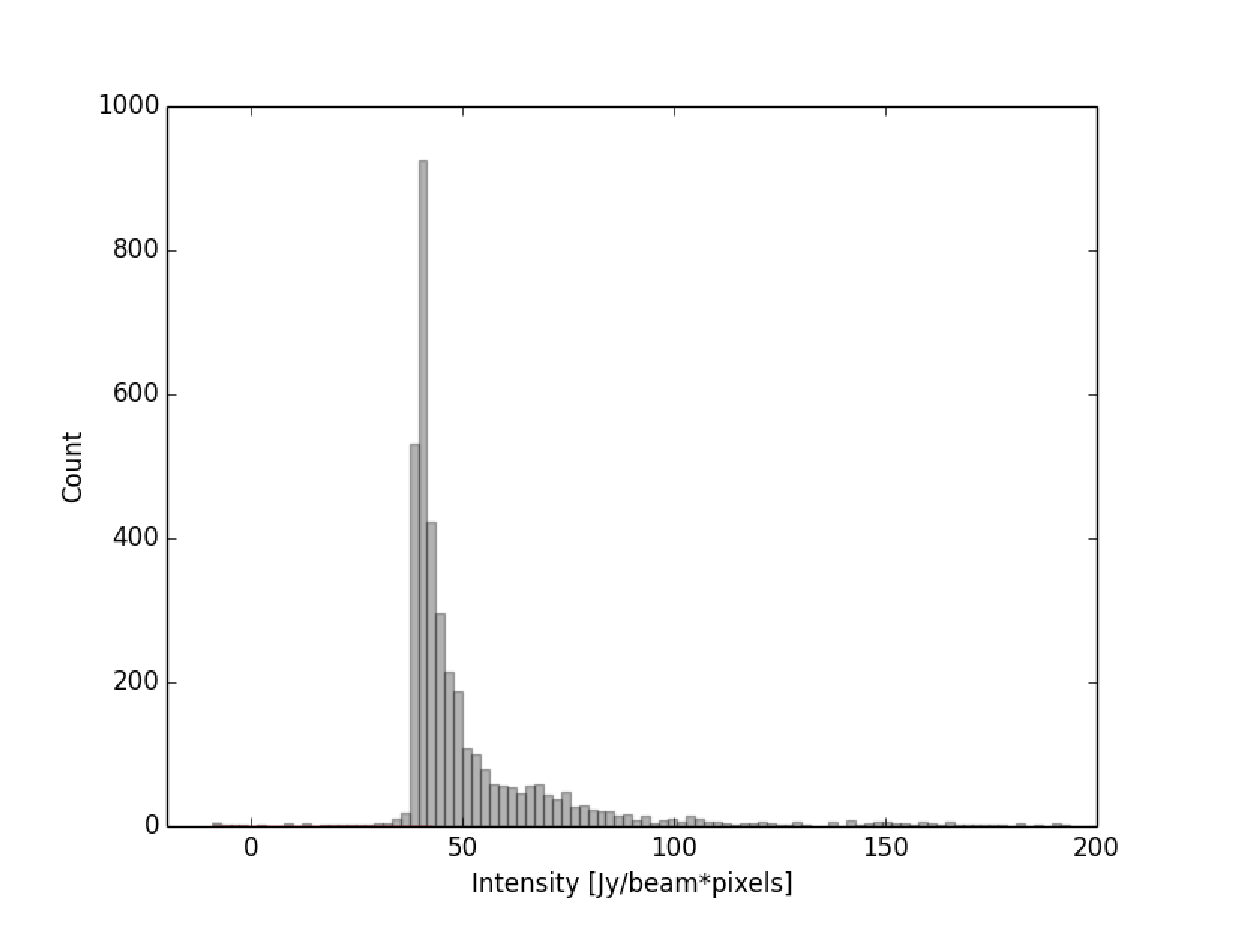
\includegraphics[width=0.98\textwidth]{OrionKL/ex_histogram.eps}
%\\(a) 左の図の説明
%\end{center}
%\end{minipage}
%\begin{minipage}{0.48\textwidth}
%\begin{center}
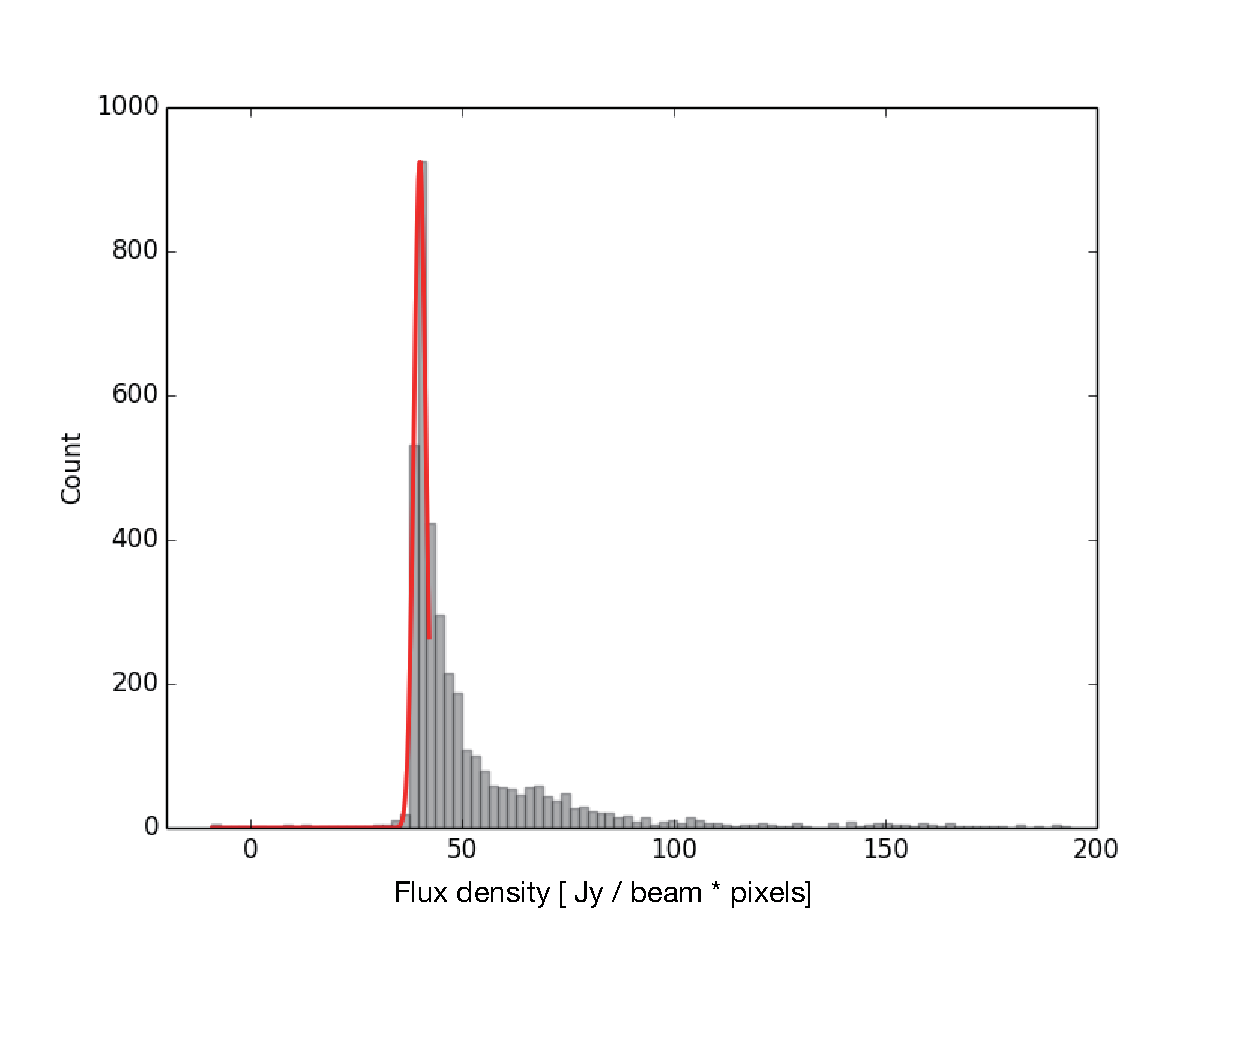
\includegraphics[width=0.8\textwidth]{OrionKL/ex_histogram_fit.eps}
%\\(b) 右の図の説明
%\end{center}
%\end{minipage}
%\end{center}
%\end{minipage}
\caption{Schematic description of the process of determination of the continuum level toward Orion-KL: 
shown are the flux distributions of Hot core (histogram) with the resulting fit overlaid (red line).}
\end{center}
\end{figure}



\begin{figure}[htbp]
  \centering
  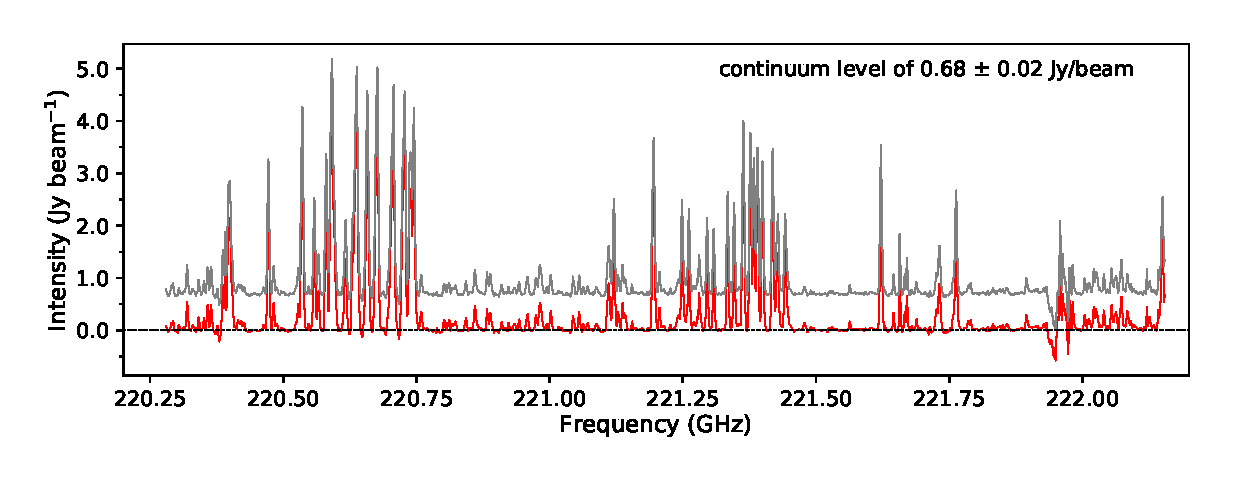
\includegraphics[width=0.98\textwidth]{OrionKL/spec_spw2.eps}
  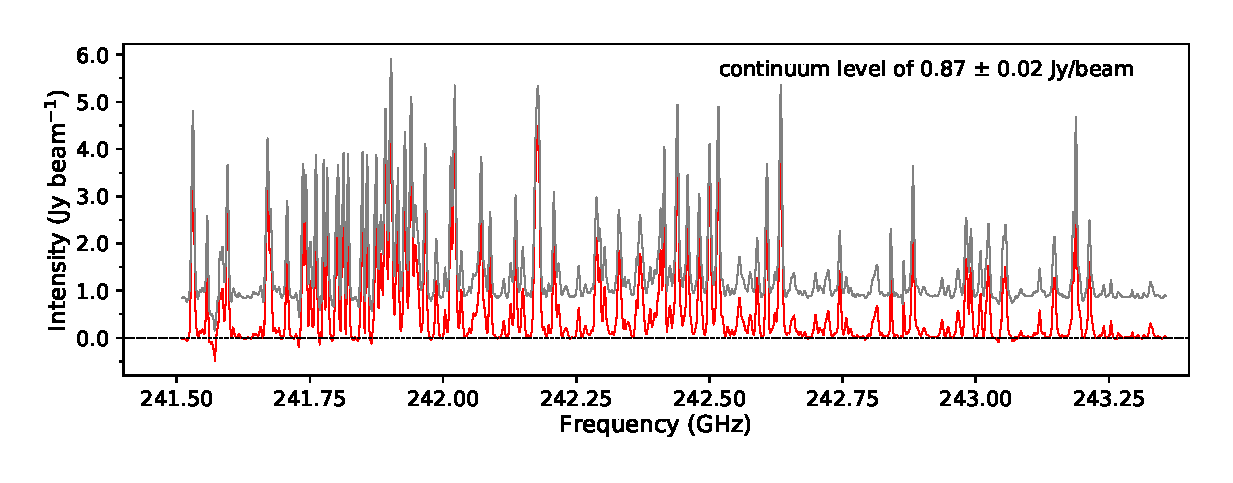
\includegraphics[width=0.98\textwidth]{OrionKL/spec_spw13.eps}
  \caption{The original spectra (gray) and continuum-subtracted spectra (red) towards Hot core. 
  The continuum emission level subtracted to the original spectra, together with its uncertainty,
  is listed in the upper right part of each panel.}
  \label{SVspec}
\end{figure}



\subsection{Line identification}

We drew CH$_{3}$NH$_{2}$ emission maps using Common Astronomy Software Applications 
(CASA) software \citep{McMullin+2007}.
We used JPL Molecular Spectroscopy catalog to identify the transition lines. 
8 spectral features exhibit a compact emission at the center of the Hot core . 
We extracted spectrum from this region.
Possible line blending with CH$_{3}$NH$_{2}$ was investigated by JPL database\footnote{http://spec.jpl.nasa.gov}, 
the Cologne database for molecular spectroscopy (CDMS)\footnote{http://www.astro.uni-koeln.de/cdms/}, 
and Splatalogue\footnote{http://www.splalogue.net/}. 

2. We estimated the systemic velocity and the line width of 217.758 GHz line, 
reported by Pagani et al. (2017), which seem contaminated by 
other lines.

3. Using these value, we obtained the integrated 
intensity of 8 transitions described in Table \ref{tab_MAOri} by Gaussian fitting.



\section{Results}
\subsection{Transitions}
The data obtained for  CH$_{3}$NH$_{2}$ are summarized in Table \ref{tab_MAOri}.
Here the rest frequencies, $S\mu^2$, upper state energy ($E_{\mathrm{u}}$), the quantum numbers,
noise level, and peak brightness temperature are given.
Out of 32 predicted transitions ($S\mu^2 > 25\,\mathrm{D^2}$ and $E_{\mathrm{u}} < 200 \,\mathrm{K}$) 
in our observational frequency range, 6 were probably identified in this data set, and are reported in
Table \ref{tab_MAOri}. The remaining 18 CH$_{3}$NH$_{2}$ transitions are
blended with or masked by other spectral features, or its signal are below the noise level 
(See Appendix A). 

\renewcommand{\arraystretch}{1.5}
\begin{table}[htb]
\begin{center}

  \caption{Observed rotational transitions of CH$_3$NH$_2$ in Orion-KL}
  \label{tab_MAOri}
{\scriptsize
  \begin{tabular}{ccccccl} \hline
   Fequency [GHz]& S$\mu ^{2}$ [D$^2$] & E$_{\rm{u}}$ [K]& Transition ($J$, $K_{\rm{a}}$, $\Gamma$) & Noise [K] & peak $T_{\mathrm{B}} [K]$ &Comments \\ \hline 
%    215.670 & 53.92 & 111.48 & 9, 2, $E_{1-1}$ $\rightarrow$ 9, 1, $E_{1+1}$ && &  \\
    245.202 & 37.84 & 168.31 & 12, 1, $B_{2}$ $\rightarrow$ 11, 2, $B_{1}$ & &&Reported in Pagani+17 \\
    217.758 & 129.88 & 182.05 & 12, 2, $B_{2}$ $\rightarrow$ 12, 1, $B_{1}$ &&&Reported in Pagani+17 \\
%    221.755 & 35.06 & 133.11 & 10, 2, $A_{2}$ $\rightarrow$ 10, 1, $A_{1}$ &&&SV data \\
    229.908 & 27.37 & 92.71 & 8, 2, $A_{2}$ $\rightarrow$ 8, 1, $A_{1}$ & &&\\ 
    235.735 & 82.06 & 92.76 & 8, 2, $B_{2}$ $\rightarrow$ 8, 1, $B_{1}$ &&&Reported in Pagani+17 \\
    242.262 & 60.23 & 60.86 & 6, 2, $B_{2}$ $\rightarrow$ 6, 1, $B_{1}$ &&&SV data \\
    244.887 & 49.54 & 48.09 & 5, 2, $B_{1}$ $\rightarrow$ 5, 1, $B_{2}$ &&&Reported in Pagani+17 \\ \hline
  \end{tabular}
  }
\end{center}
\end{table}

\subsection{Distribution}

%%%%% 積分強度図挿入 %%%%%
\begin{figure}[H] 
\begin{center}
\begin{minipage}{0.98\textwidth} 
\begin{center}
%%%% ここから
\begin{minipage}{0.48\textwidth}
\begin{center}
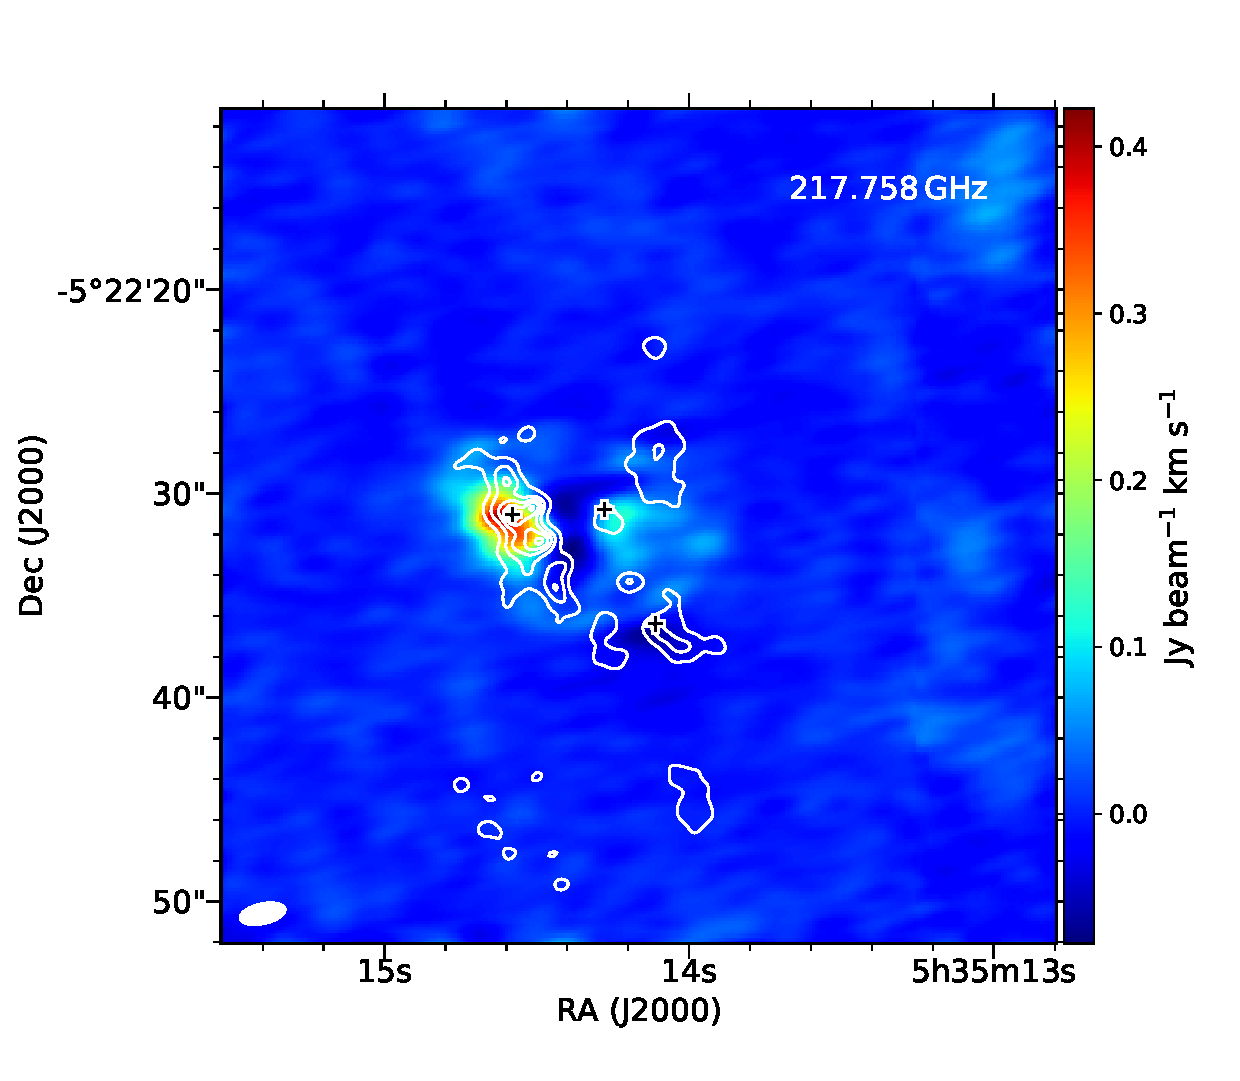
\includegraphics[width=0.98\textwidth]{OrionKL/mom0/217.758mom0_3-7.eps}
%\\(a) 左の図の説明
\end{center}
\end{minipage}
\begin{minipage}{0.48\textwidth}
\begin{center}
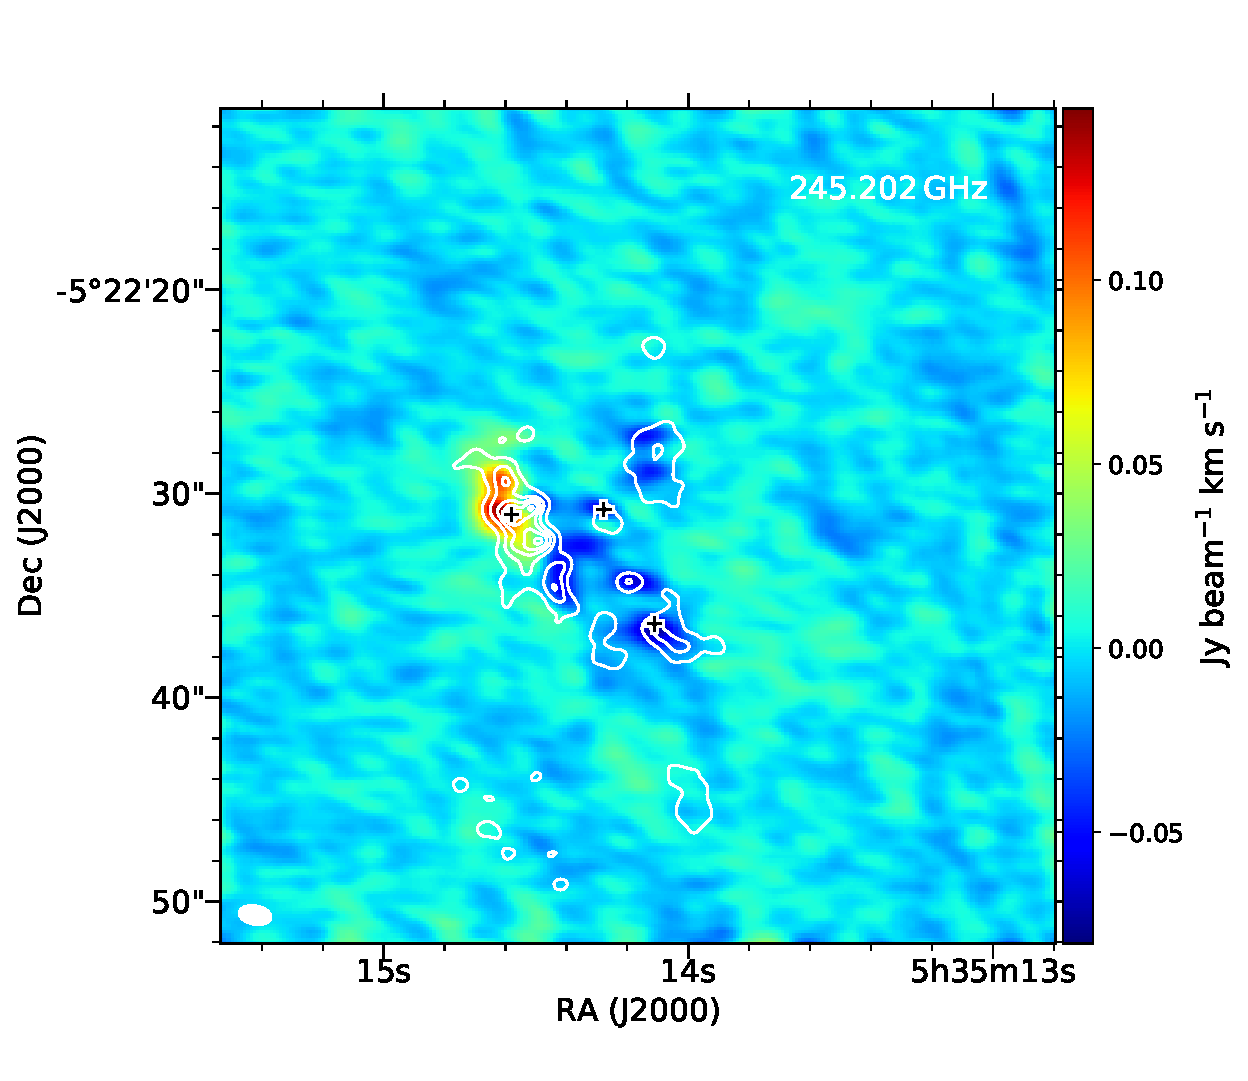
\includegraphics[width=0.98\textwidth]{OrionKL/mom0/245.202mom0_3-7.eps}
%\\(b) 右の図の説明
\end{center}
\end{minipage}
\end{center}
\end{minipage}
%%%% ここまで一組

%\begin{minipage}{0.98\textwidth} 
%\begin{center}
%\begin{minipage}{0.48\textwidth}
%\begin{center}
%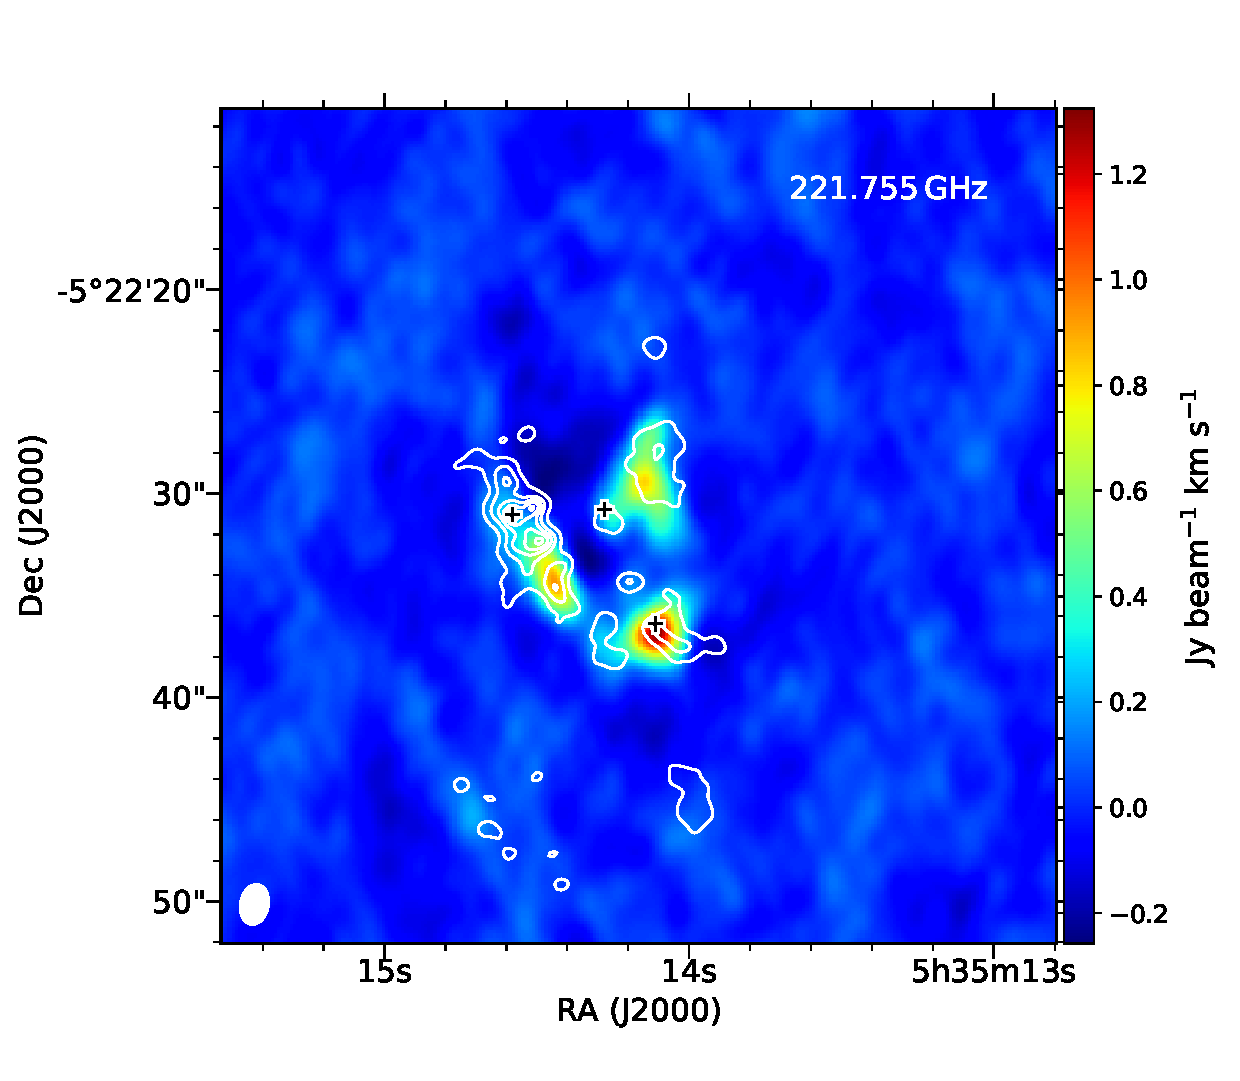
\includegraphics[width=0.98\textwidth]{OrionKL/mom0/221.755SV_mom0_3-7.eps}
%\\(c) 左の図の説明
%\end{center}
%\end{minipage}
%\begin{minipage}{0.48\textwidth}
%\begin{center}
%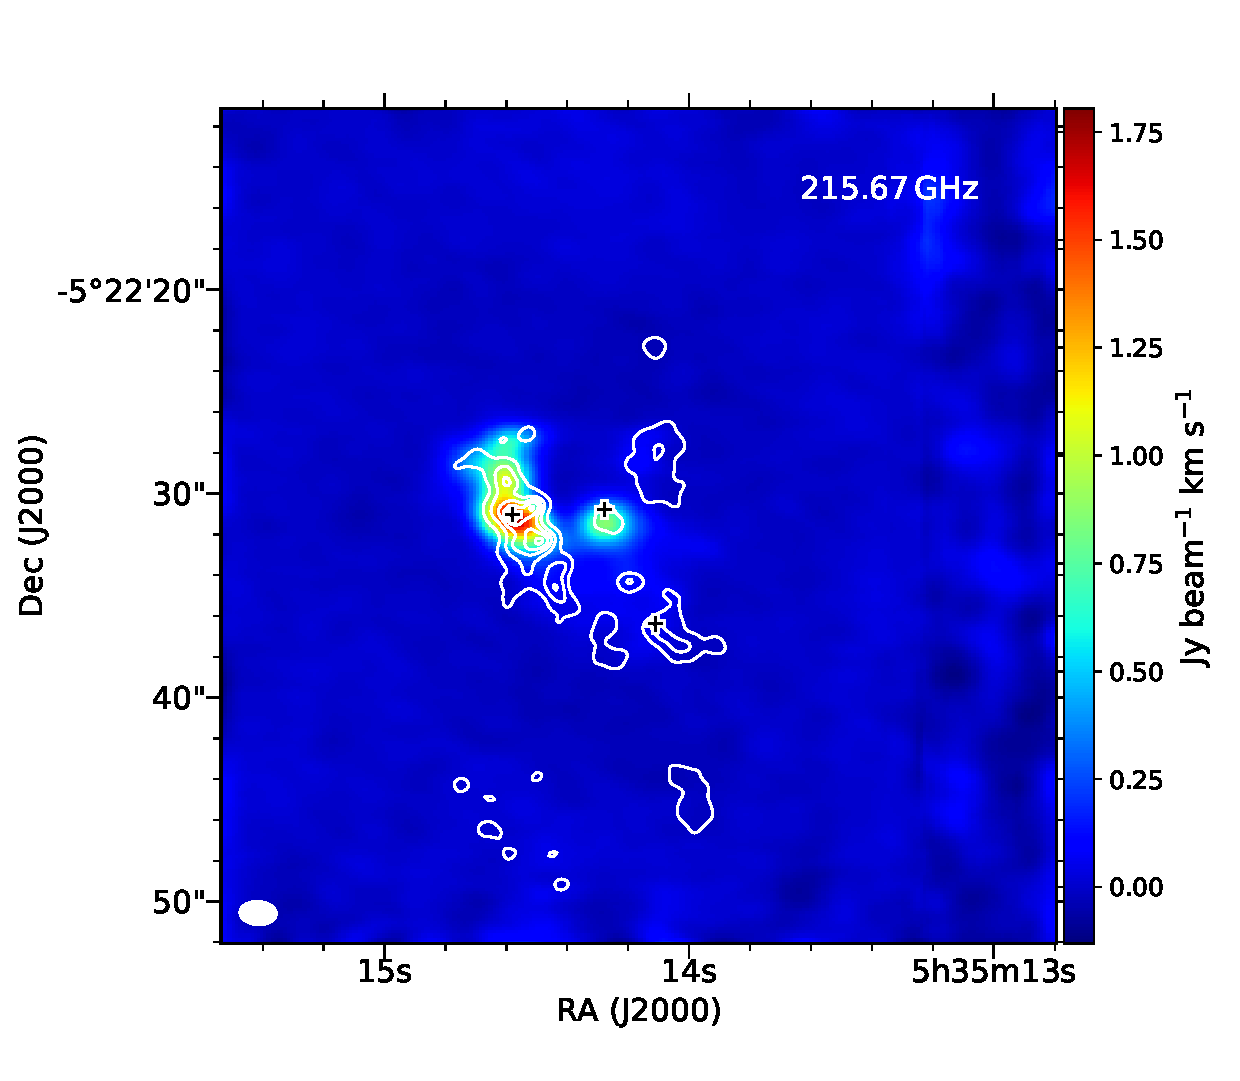
\includegraphics[width=0.98\textwidth]{OrionKL/mom0/215.67mom0_3-7.eps}
%\\(d) 右の図の説明
%\end{center}
%\end{minipage}
%\end{center}
%\end{minipage}

\caption{Integrated intensity maps of unblended CH$_{3}$NH$_{2}$ lines. 
The white contours show the 1.3 mm continuum map from \citet{Hirota+2015},
where the contour levels are 10 \%, 30 \%, 50 \%, 70 \%, 90 \% of the peak intensity.
Black crosses denote Hot core, IRc7, and Compact ridge. 
The rest frequency of each transition shows in the upper right part of each panel.}
\end{center}
\end{figure}

\newpage

\begin{figure}[H] 
\begin{center}
\begin{minipage}{0.98\textwidth} 
\begin{center}
%%%% ここから
\begin{minipage}{0.48\textwidth}
\begin{center}
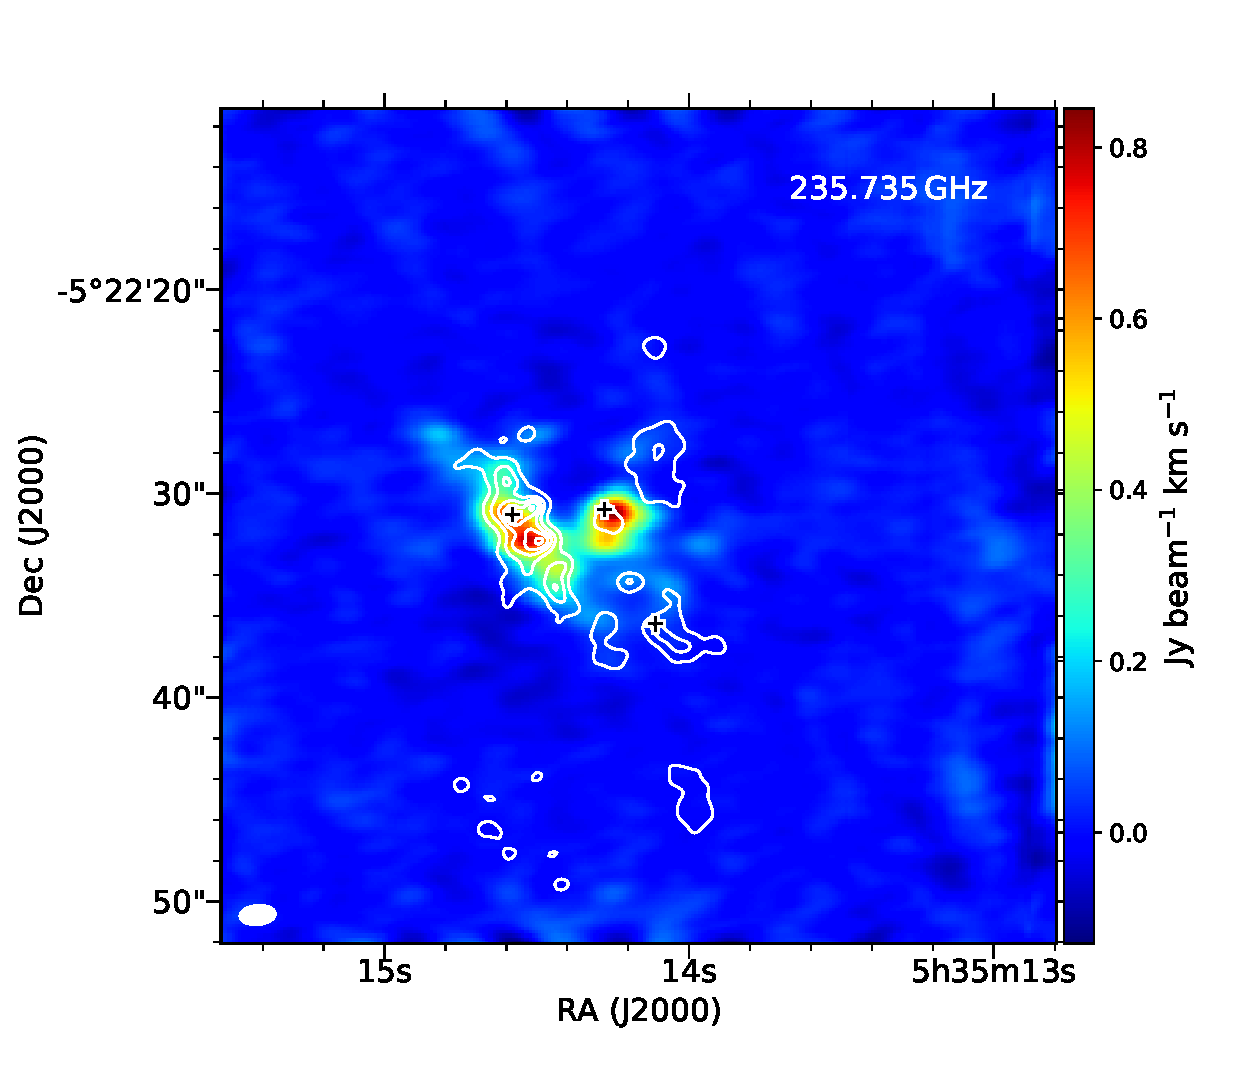
\includegraphics[width=0.98\textwidth]{OrionKL/mom0/235.735mom0_3-7.eps}
%\\(e) 左の図の説明
\end{center}
\end{minipage}
\begin{minipage}{0.48\textwidth}
\begin{center}
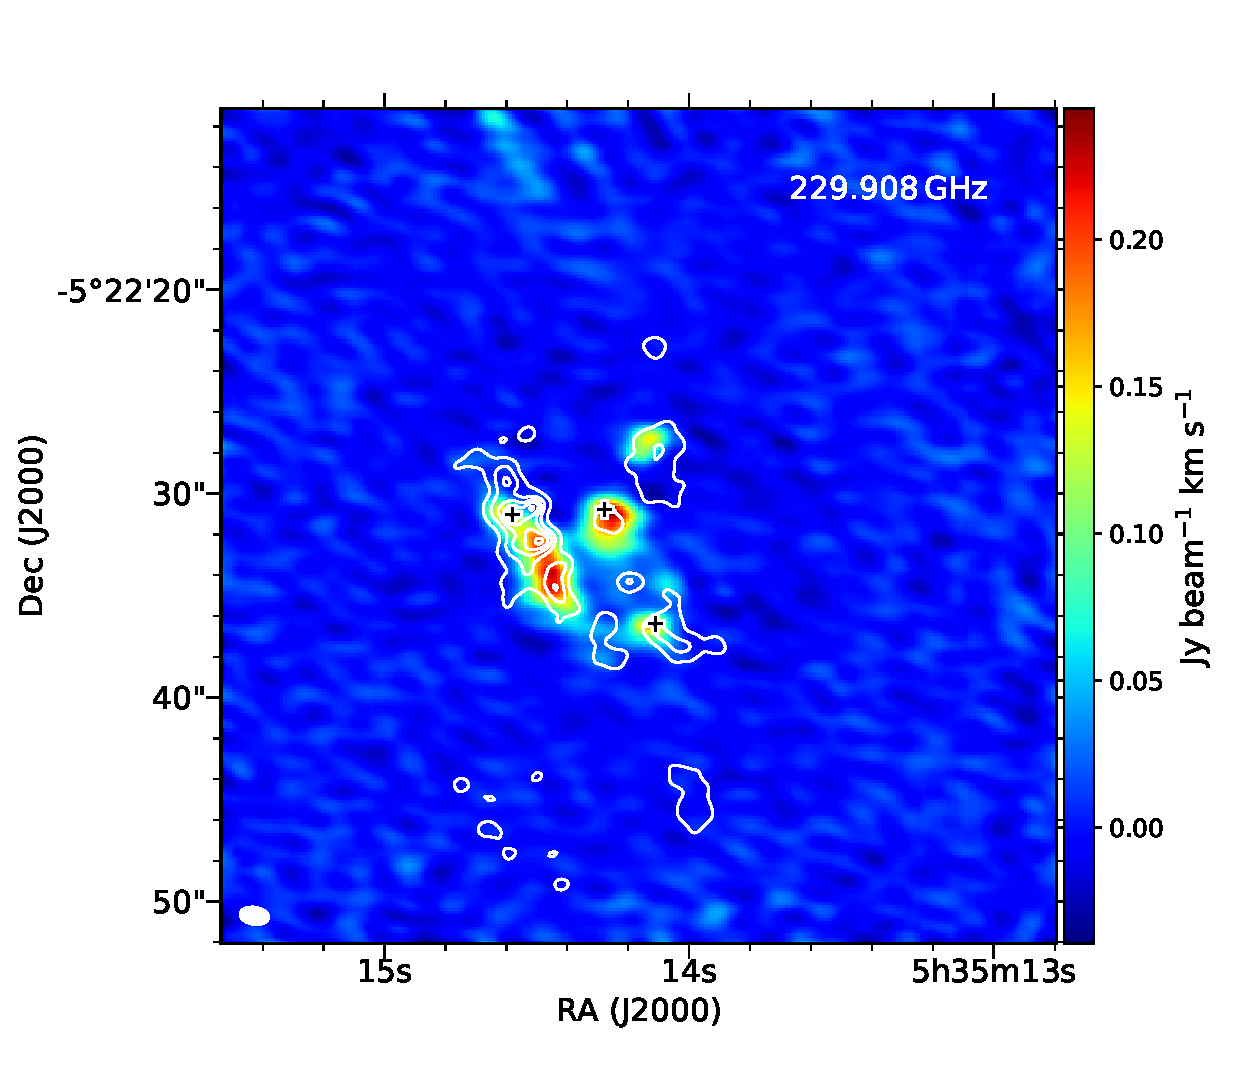
\includegraphics[width=0.98\textwidth]{OrionKL/mom0/229.908mom0_3-7.eps}
%\\(f) 右の図の説明
\end{center}
\end{minipage}
\end{center}
\end{minipage}
%%%% ここまで一組

\begin{minipage}{0.98\textwidth} 
\begin{center}
\begin{minipage}{0.48\textwidth}
\begin{center}
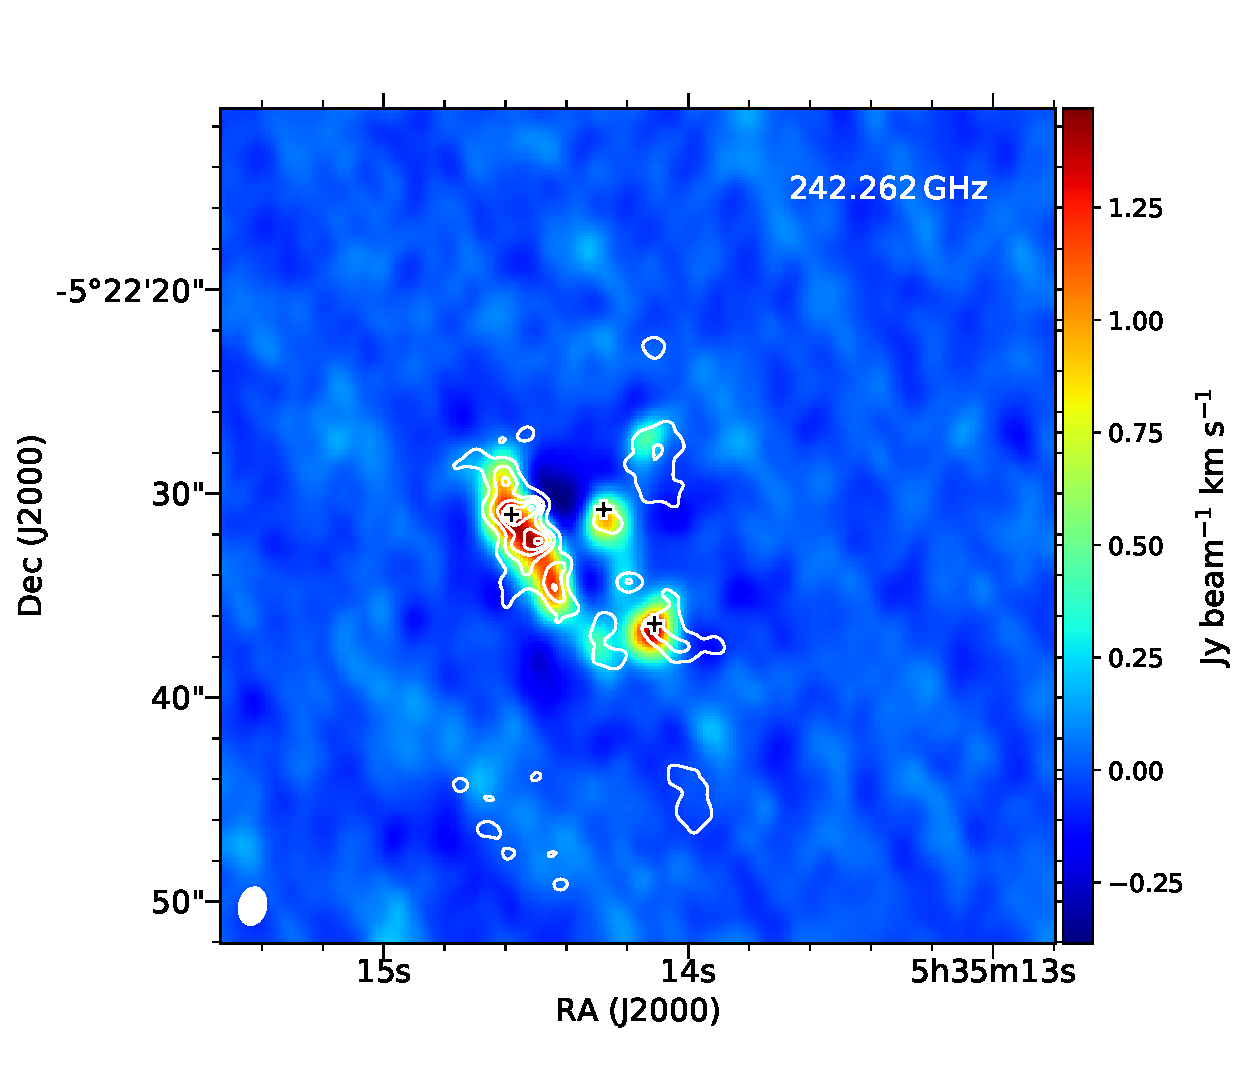
\includegraphics[width=0.98\textwidth]{OrionKL/mom0/242.262SV_mom0_3-7.eps}
%\\(g) 左の図の説明
\end{center}
\end{minipage}
\begin{minipage}{0.48\textwidth}
\begin{center}
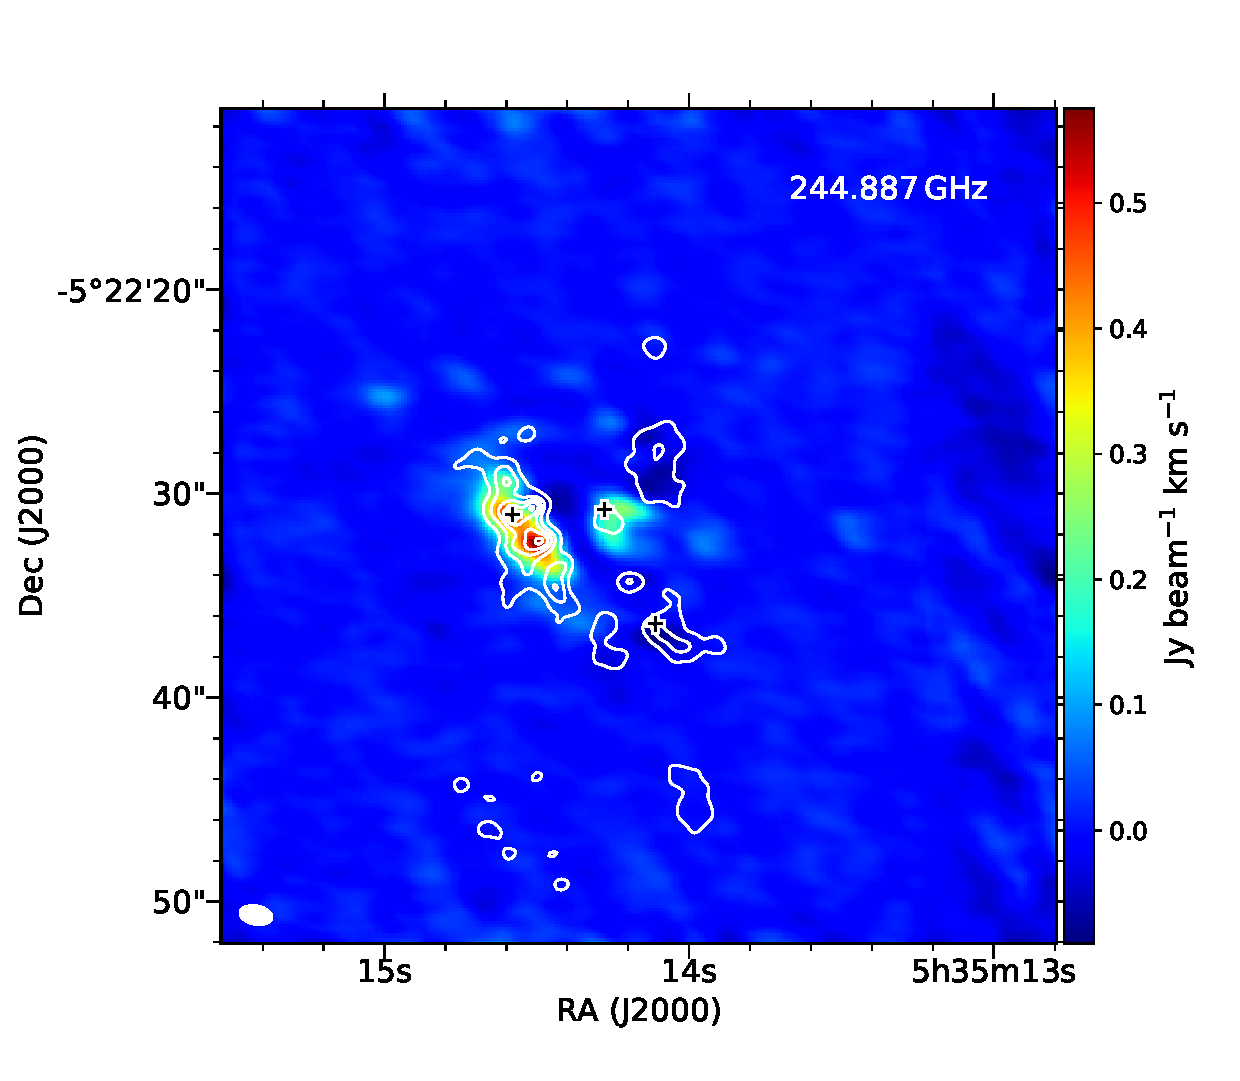
\includegraphics[width=0.98\textwidth]{OrionKL/mom0/244.887mom0_3-7.eps}
%\\(h) 右の図の説明
\end{center}
\end{minipage}
\end{center}
\end{minipage}

\caption{(Continued)}
\end{center}
\end{figure}
%%%%% 積分強度図ここまで %%%%%

%%%%%% チャネルマップここから
\begin{figure}[H]
  \centering
  \includegraphics[width=0.98\textwidth]{OrionKL/chmap/217.758.eps}
  \caption{
  Channel map of expected unblended 217.758 GHz line show multiple velocity-dependent 
  emission peaks: 4-6 km s$^{-1}$ towards Hot core, 7-9km s$^{-1}$ towards IRc7. 
  Magenta crosses denote Hot core, IRc7, and Compact ridge.}
  \label{ch_0}
\end{figure}

\begin{figure}[H]
  \centering
  \includegraphics[width=0.98\textwidth]{OrionKL/chmap/245.202.eps}
  \caption{Channel map of expected unblended 245.202 GHz line.}
  \label{ch_1}
\end{figure}

\begin{figure}[H]
  \centering
  \includegraphics[width=0.98\textwidth]{OrionKL/chmap/235.735.eps}
  \caption{Channel map of expected unblended 235.735 GHz line.}
  \label{ch_2}
\end{figure}

\begin{figure}[H]
  \centering
  \includegraphics[width=0.98\textwidth]{OrionKL/chmap/242.262.eps}
  \caption{Channel map of expected unblended 242.262 GHz line.}
  \label{ch_3}
\end{figure}

%\begin{figure}[H]
%  \centering
%  \includegraphics[width=0.98\textwidth]{OrionKL/chmap/215.67.eps}
%  \caption{Channel map of expected unblended 215.670 GHz line.}
%  \label{ch_4}
%\end{figure}

\begin{figure}[H]
  \centering
  \includegraphics[width=0.98\textwidth]{OrionKL/chmap/244.887.eps}
  \caption{Channel map of expected unblended 244.887 GHz line.}
  \label{ch_5}
\end{figure}

%\begin{figure}[H]
%  \centering
%  \includegraphics[width=0.98\textwidth]{OrionKL/chmap/221.755.eps}
%  \caption{Channel map of expected unblended 221.755 GHz line.}
%  \label{ch_6}
%\end{figure}

\begin{figure}[H]
  \centering
  \includegraphics[width=0.98\textwidth]{OrionKL/chmap/229.908.eps}
  \caption{Channel map of expected unblended 229.908 GHz line.}
  \label{ch_7}
\end{figure}

\subsection{Spectrum}
%%%%% スペクトル挿入 %%%%%
\begin{figure}[H] 
\begin{center}
\begin{minipage}{0.98\textwidth} 
\begin{center}
%%%% ここから
\begin{minipage}{0.48\textwidth}
\begin{center}
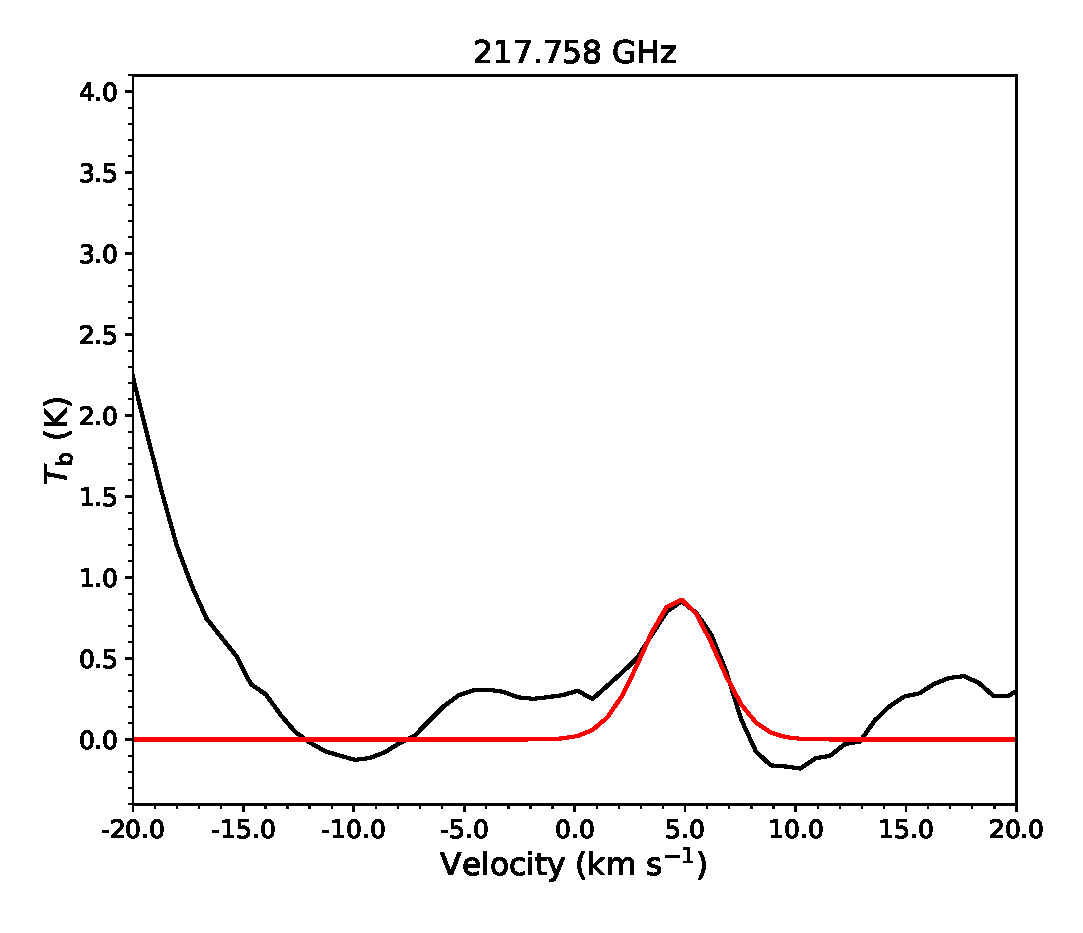
\includegraphics[width=0.98\textwidth]{OrionKL/spectrum/HC/217.758328w_fit.eps}
%\\(a) 左の図の説明
\end{center}
\end{minipage}
\begin{minipage}{0.48\textwidth}
\begin{center}
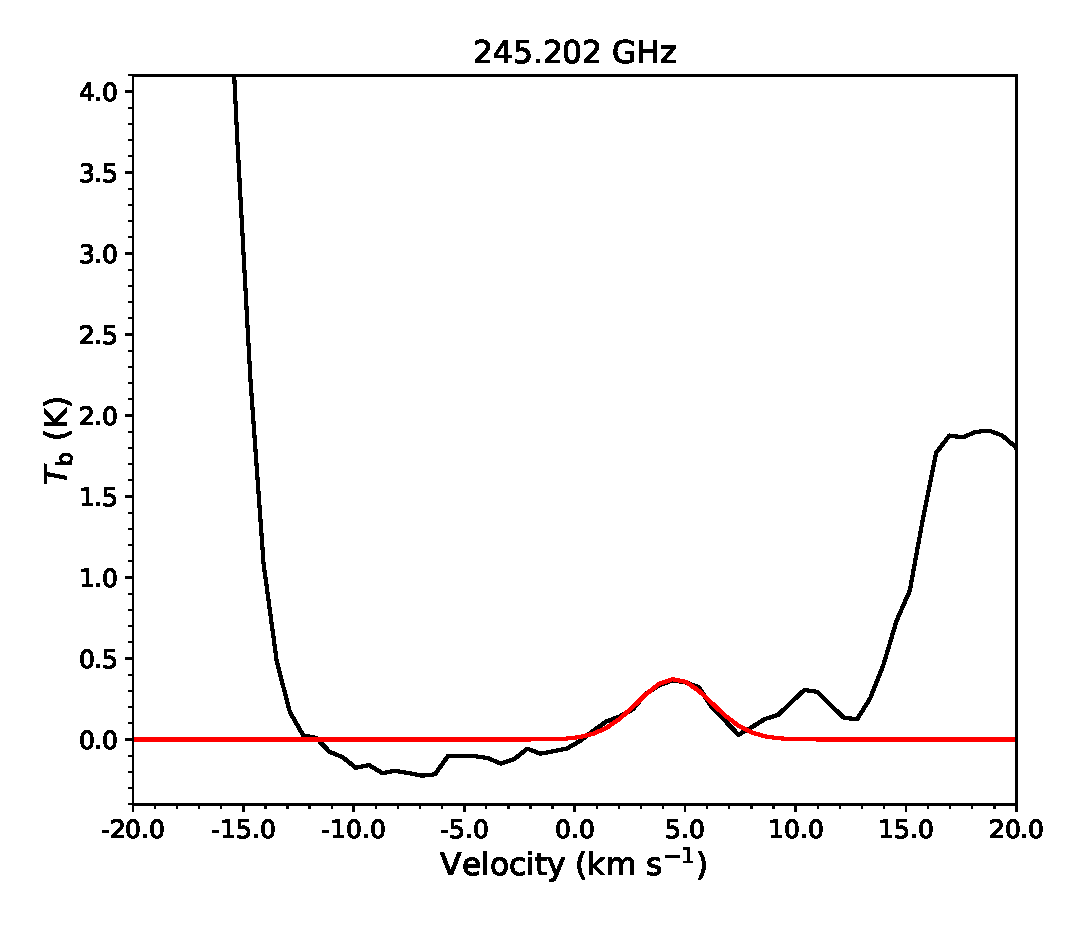
\includegraphics[width=0.98\textwidth]{OrionKL/spectrum/HC/245.2021362w_fit.eps}
%\\(b) 
\end{center}
\end{minipage}
\end{center}
\end{minipage}
%%%% ここまで一組

%\begin{minipage}{0.98\textwidth} 
%\begin{center}
%\begin{minipage}{0.48\textwidth}
%\begin{center}
%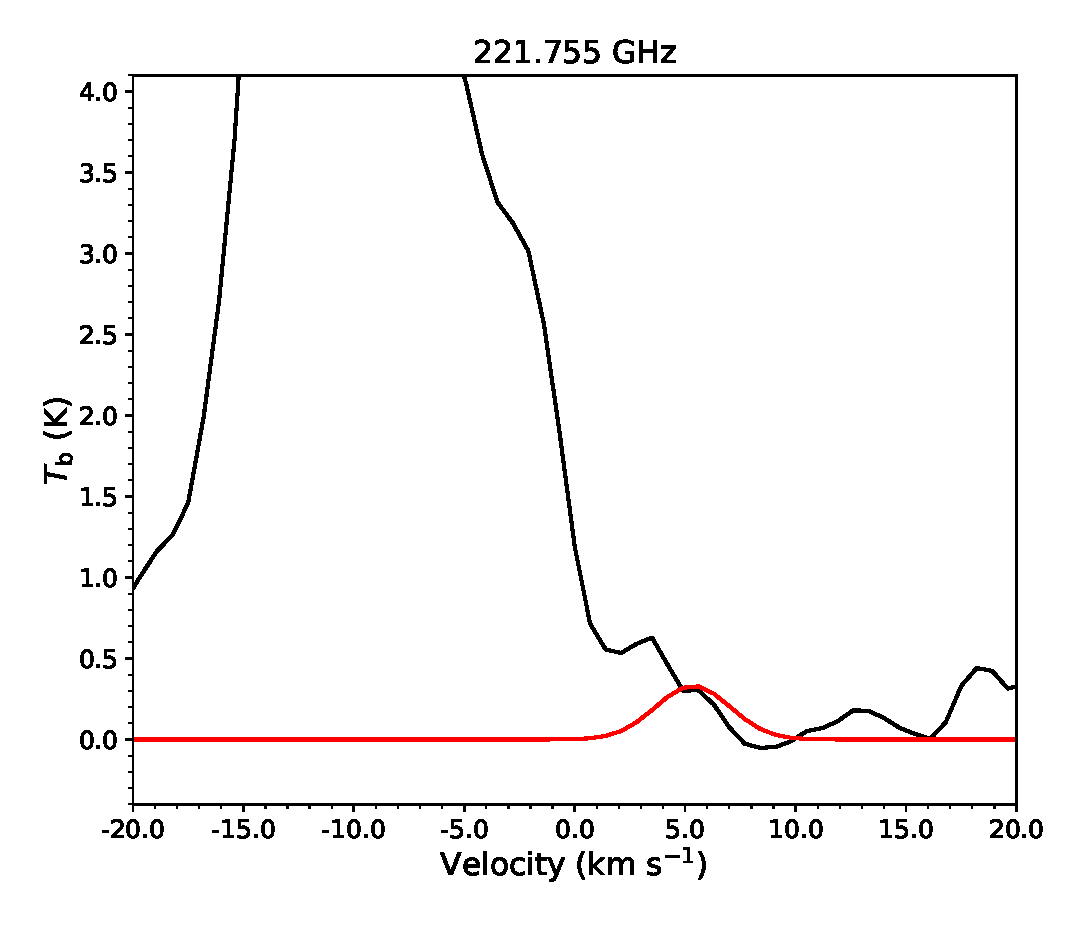
\includegraphics[width=0.98\textwidth]{OrionKL/spectrum/HC/221.755055w_fit.eps}
%\\(c) 左の図の説明
%\end{center}
%\end{minipage}
%\begin{minipage}{0.48\textwidth}
%\begin{center}
%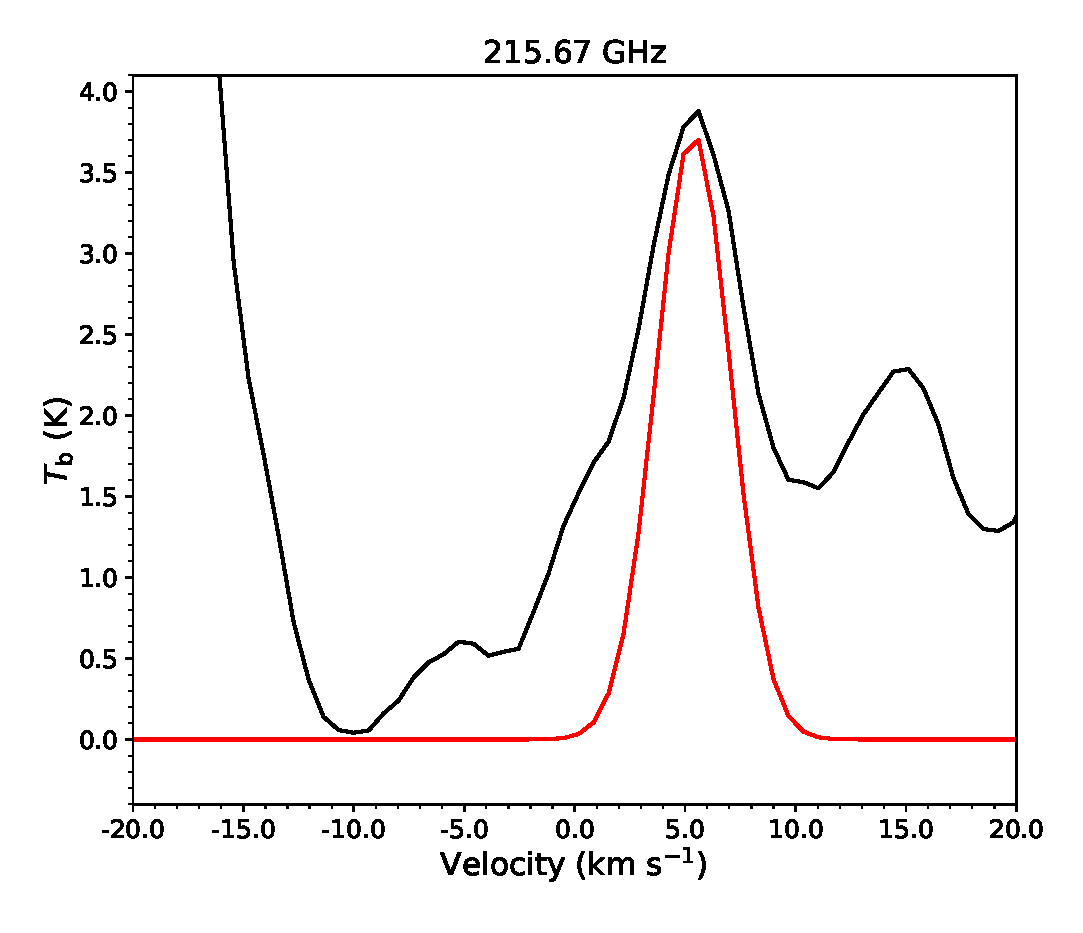
\includegraphics[width=0.98\textwidth]{OrionKL/spectrum/HC/215.6696452w_fit.eps}
%\\(d) 右の図の説明
%\end{center}
%\end{minipage}
%\end{center}
%\end{minipage}
\begin{minipage}{0.98\textwidth} 
\begin{center}
%%%% ここから
\begin{minipage}{0.48\textwidth}
\begin{center}
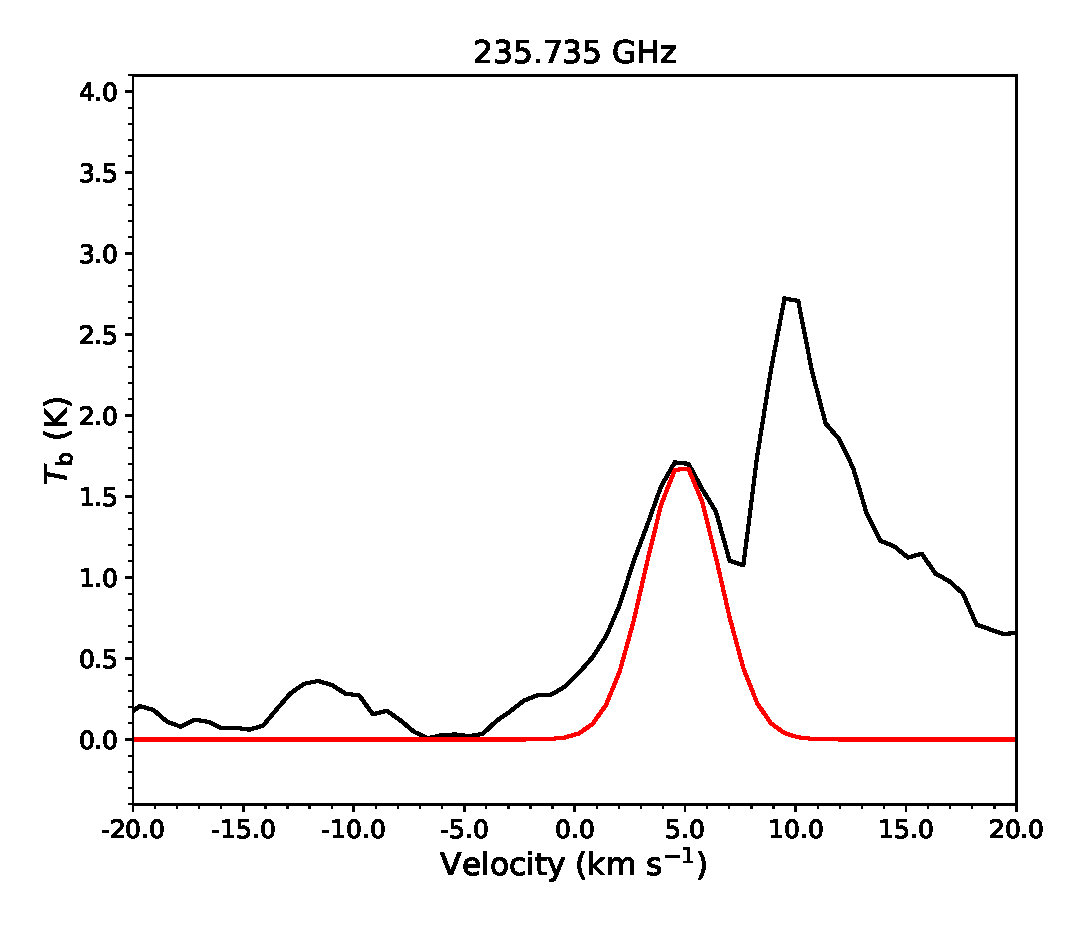
\includegraphics[width=0.98\textwidth]{OrionKL/spectrum/HC/235.735037w_fit.eps}
%\\(e) 左の図の説明
\end{center}
\end{minipage}
\begin{minipage}{0.48\textwidth}
\begin{center}
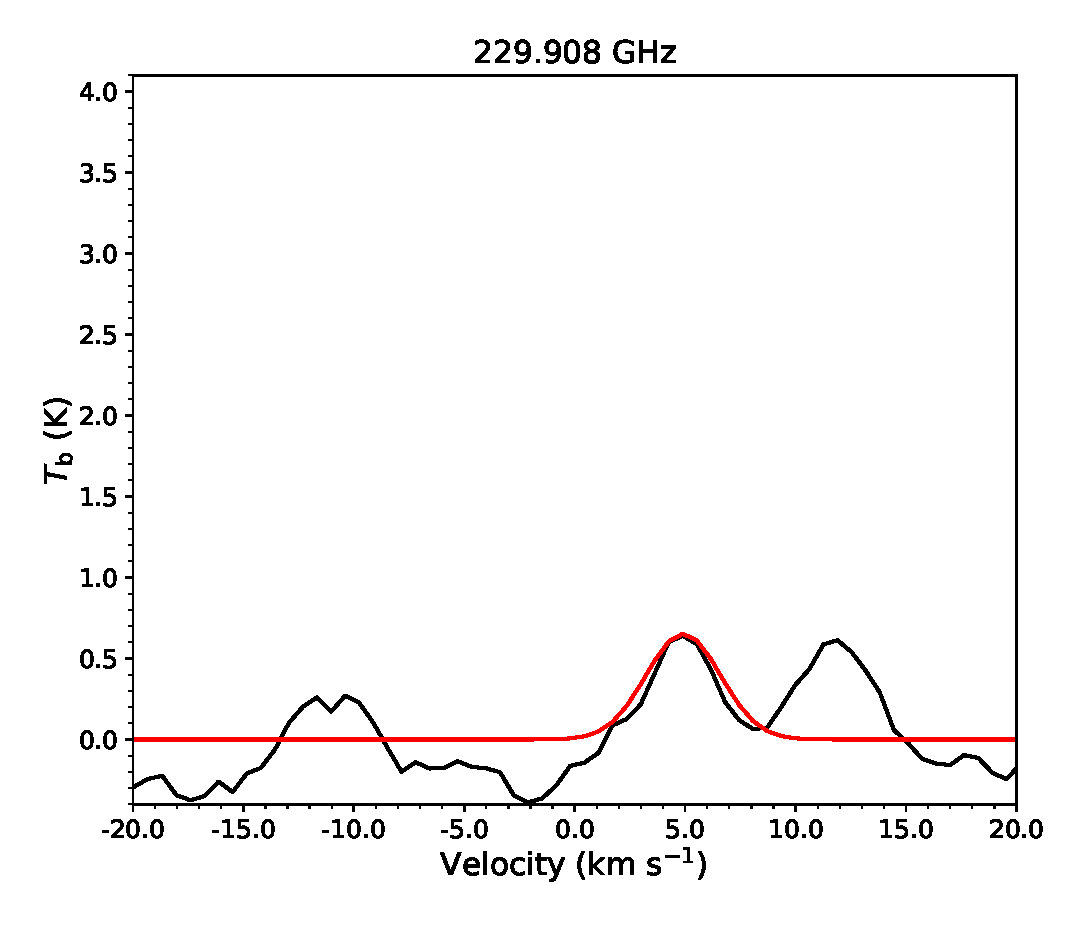
\includegraphics[width=0.98\textwidth]{OrionKL/spectrum/HC/229.908118w_fit.eps}
%\\(f) 右の図の説明
\end{center}
\end{minipage}
\end{center}
\end{minipage}
%%%% ここまで一組

\begin{minipage}{0.98\textwidth} 
\begin{center}
\begin{minipage}{0.48\textwidth}
\begin{center}
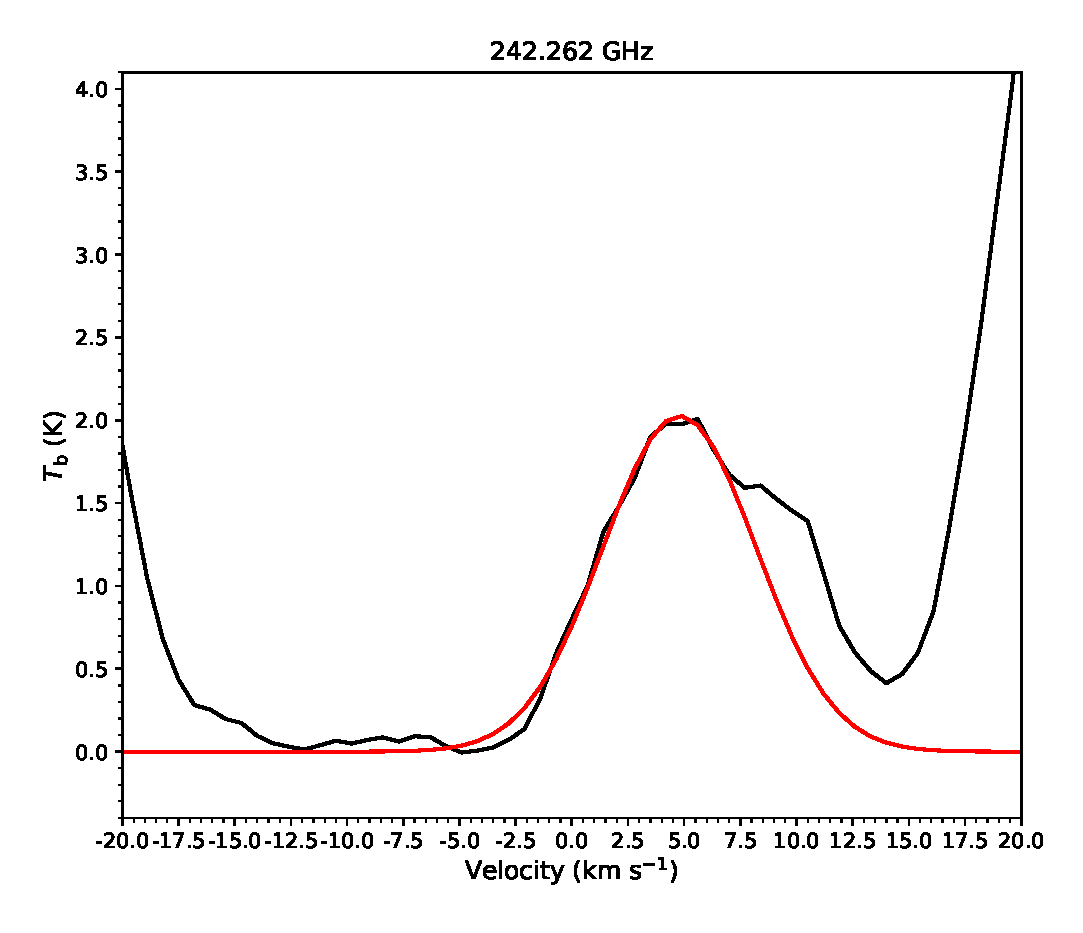
\includegraphics[width=0.98\textwidth]{OrionKL/spectrum/HC/242.2620195w_fit.eps}
%\\(g) 左の図の説明
\end{center}
\end{minipage}
\begin{minipage}{0.48\textwidth}
\begin{center}
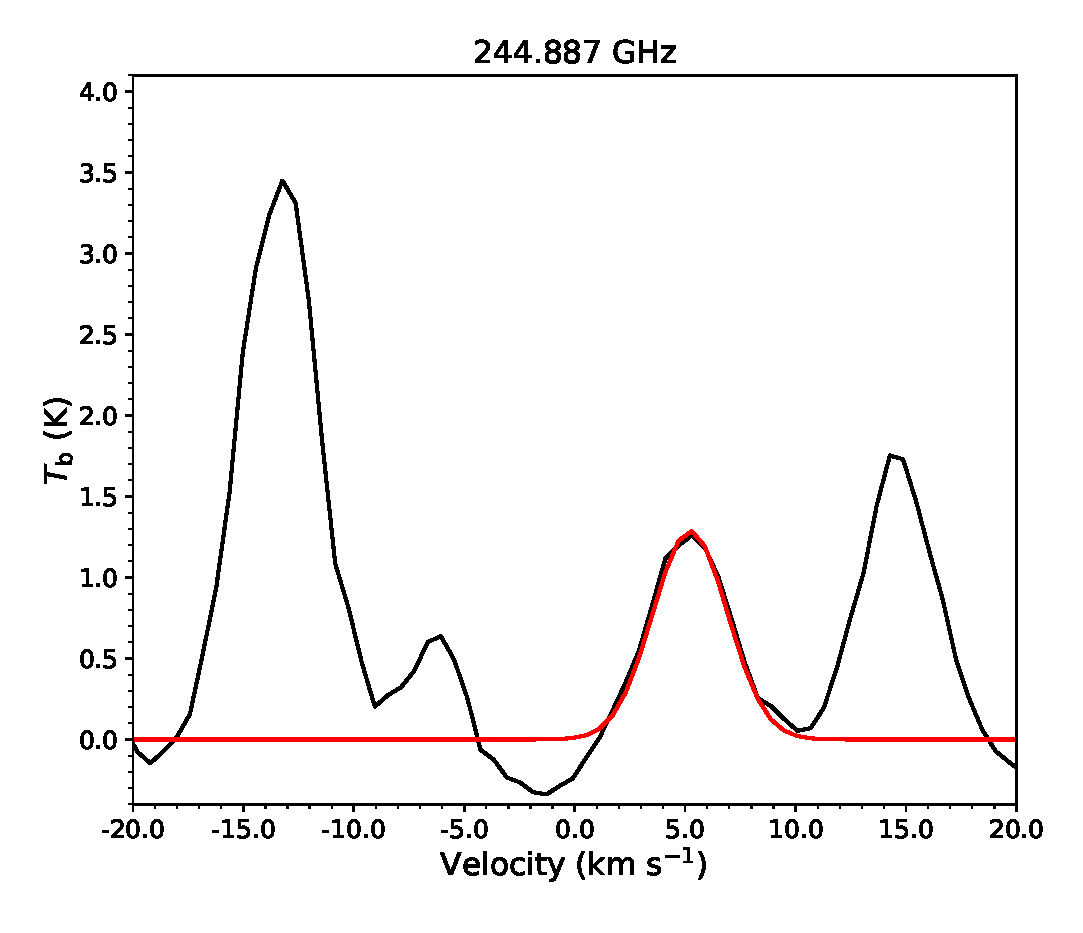
\includegraphics[width=0.98\textwidth]{OrionKL/spectrum/HC/244.8869007w_fit.eps}
%\\(h) 右の図の説明
\end{center}
\end{minipage}
\end{center}
\end{minipage}

\caption{Spectrum of the CH$_3$NH$_2$ lines at each frequency observed in Hot core center (black) 
  and the result of the Gaussian fitting (red).}
\end{center}
\end{figure}


\section{Disucssion}
\subsection{Column density and Rotation temperature}

In this subsection we will describe the methodologies in deriving fractional abundances of COMs.
The column density of CH$_{3}$NH$_{2}$ ($N_{\mathrm{MA}}$) was established by using 
the rotational temperature diagram method, which assumes local thermodynamic equilibrium 
(LTE) and optically thin emission. 
The following equation was employed for the analysis \citep{Turner1991}:
\begin{align}
\log \dfrac{3\,k_{\mathrm{B}}\,T_{\mathrm{B}} \,\Delta V_{1/2}}{8\, \pi^3\, \nu\, S\, \mu_0^2} = \log \dfrac{N_{\mathrm{MA}}}{U_{\mathrm{rot}}} - \dfrac{E_{\mathrm{u}}}{k_{\mathrm{B}}} \dfrac{\log e}{T_{\mathrm{rot}}}
\label{eq:RD}
\end{align}

In the expression, $\nu$ is the rest frequency of the transition, $\mu_0$ is the permanent dipole moment, 
$U_{\mathrm{rot}}$ is the rotational partition function, $S$ is the line strength, 
$E_{\mathrm{u}}$ is the upper state energy, and $ T_{\mathrm{B}}$ and  $\Delta V_{1/2}$ 
are the brightness temperature and line widths (FWHM, in km s$^{-1}$), respectively.
We assumed $\Delta V_{1/2} = 4.24\, \mathrm{km\,s^{-1}}$, which derived by the Gaussian fitting for 
217.758 GHz line.

The brightness temperature can be converted from intensity $I_{\mathrm{\nu}}$
when the Rayleigh-Jeans law is applicable.
\begin{align}
T_{\mathrm{B}} = \dfrac{c^2}{2\,k_{\mathrm{B}}\, \nu^2} \,I_{\mathrm{\nu}}
\end{align}

\begin{figure}[H]
  \centering
  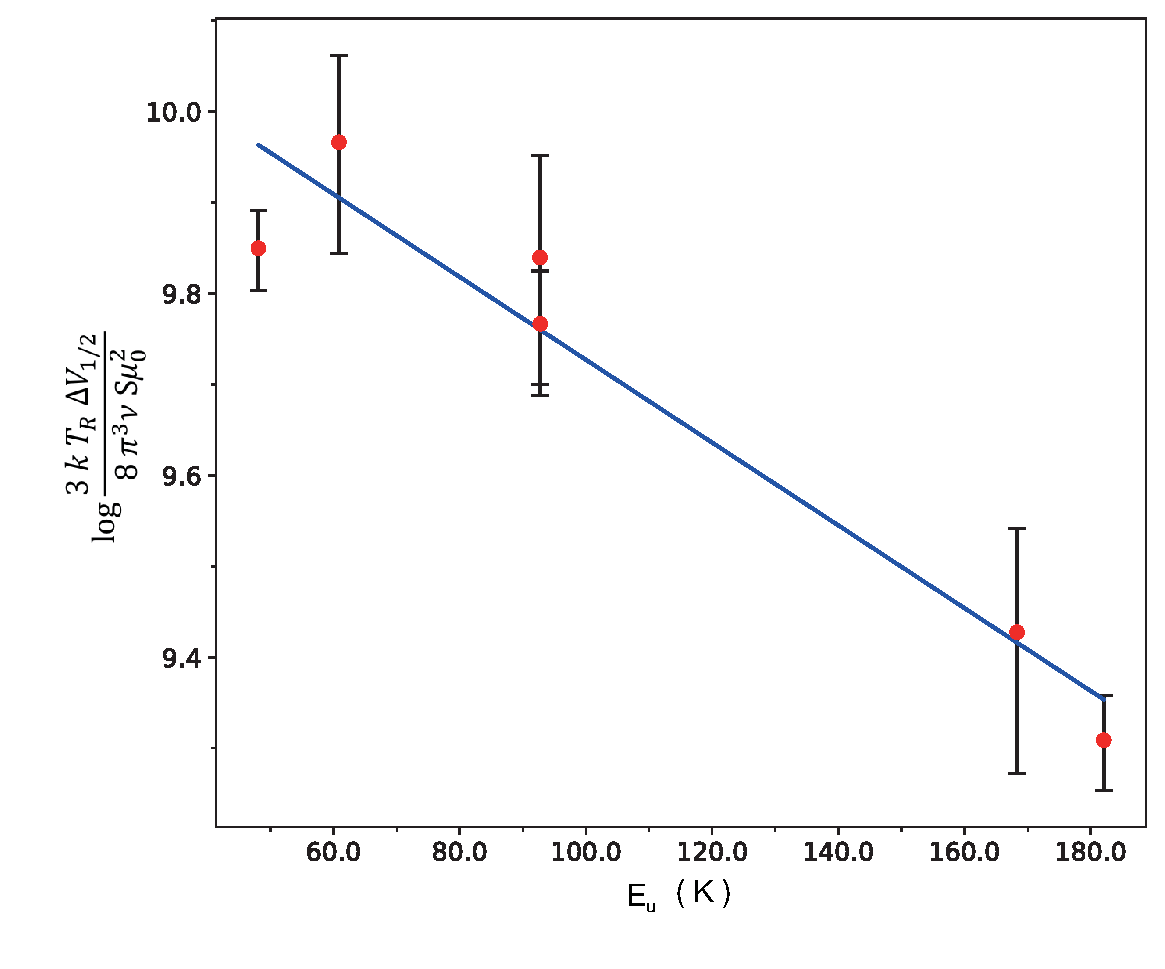
\includegraphics[width=0.8\textwidth]{OrionKL/RD_6point_label.eps}
  \caption{Rotation diagram of CH$_{3}$NH$_{2}$ in Hot core. The error bars represents $\pm$ 3 $\sigma$ for each data.}
  \label{fig:RD}
\end{figure}

The resulting plots are given in Figure \ref{fig:RD}.
The analysis yields a rotational temperature of $T_{\mathrm{rot}} =  95.4^{+15.5}_{-11.7} \,\mathrm{K}$, 
with a column density of $N_{\mathrm{MA}} = ( 5.5^{+1.6}_{-1.1} ) \times 10^{14} \,\mathrm{cm^{-2}}$.

\subsection{Blending}
As shown in Figure \ref{fig:RD_7point}, the CH$_{3}$NH$_{2}$ data produced point-to-point scatter  
perhaps because of the lower signal-to-noise ratio for the weaker transitions in SV data and 
possible low-level contamination.

\begin{figure}[H]
  \centering
  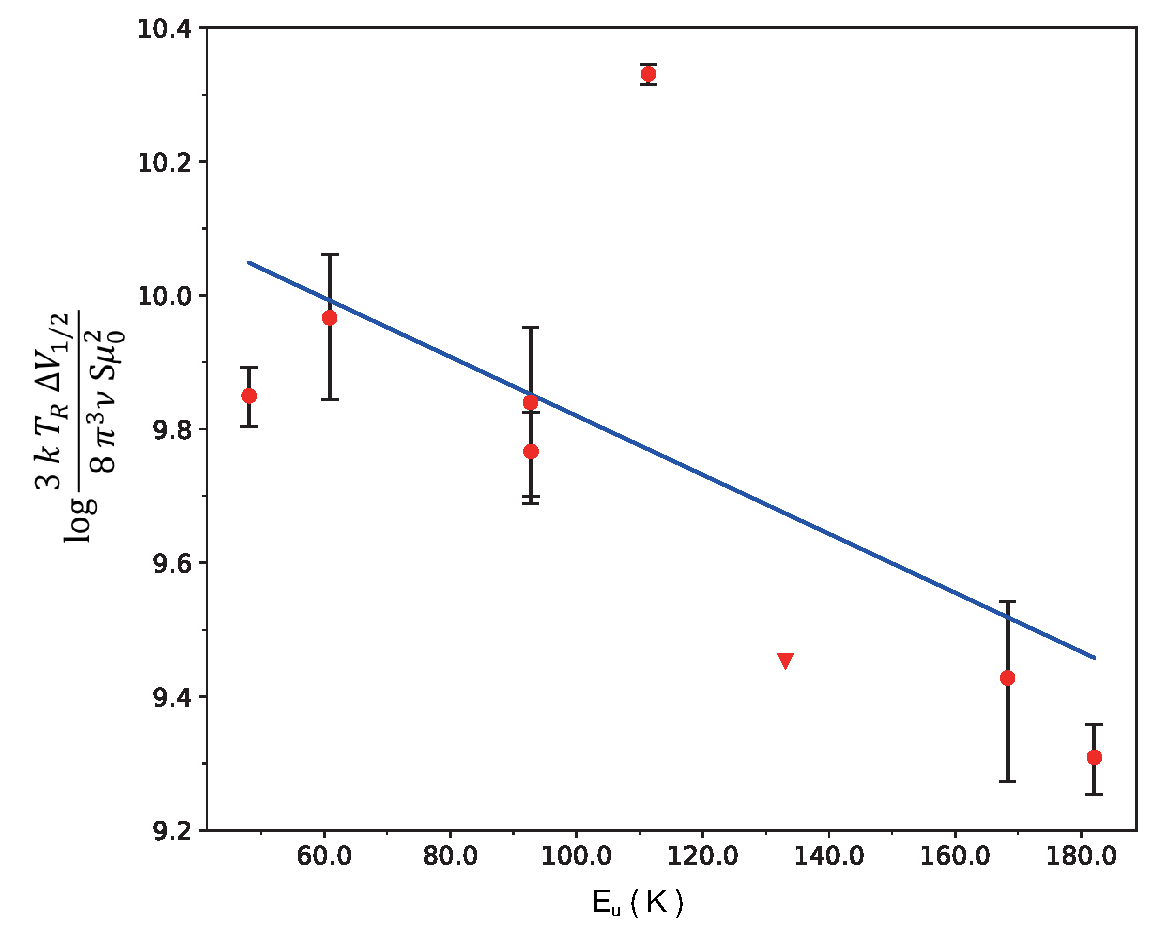
\includegraphics[width=0.8\textwidth]{OrionKL/RD_7point_label.eps}
  \caption{Rotation diagram of CH$_{3}$NH$_{2}$ in Hot core with more lines. The error bars represents $\pm$ 3 $\sigma$ for each data. Upper limit is indicated with triagle.}
  \label{fig:RD_7point}
\end{figure}